\ProvidesPackage{computer-manual}

\usepackage[utf8x]{inputenc}
\usepackage[twoside, bindingoffset=1.5cm, inner=2cm, outer=2cm, top=2cm, bottom=2cm]{geometry}
\usepackage{natbib}
\usepackage{mdwlist}
\usepackage[titles]{tocloft}
\RequirePackage{multicol}
\RequirePackage{graphicx}
\RequirePackage{textcomp}
\RequirePackage{makeidx}
\RequirePackage{wrapfig}
\RequirePackage{setspace} 
\RequirePackage[small,it]{caption}
\RequirePackage{hyperref}
\RequirePackage{parskip}
\RequirePackage{eso-pic}
\RequirePackage{listings}

%% Restyle the Table of Contents
\setlength{\cftbeforechapskip}{2ex}
\setlength{\cftbeforesecskip}{0.5ex}
\setlength{\cftbeforepartskip}{8ex}
\setlength{\cftsecnumwidth}{5ex}
\setlength{\cftsecindent}{5ex}

\renewcommand{\cftpartfont}{%
 \hfill\Large\scshape\bfseries
}


\newcommand{\version}[1]{\def\@versionnumber{#1}}



\makeindex

\hypersetup{
    bookmarks=true,         % show bookmarks bar?
    unicode=false,          % non-Latin characters in Acrobat’s bookmarks
    pdftoolbar=true,        % show Acrobat’s toolbar?
    pdfmenubar=true,        % show Acrobat’s menu?
    pdffitwindow=false,     % window fit to page when opened
    pdfstartview={FitH},    % fits the width of the page to the window
    pdftitle={Corina Manual},    % title
    pdfauthor={Peter W Brewer},     % author
    pdfsubject={Corina},   % subject of the document
    pdfnewwindow=true,      % links in new window
    colorlinks,%
    citecolor=black,%
    filecolor=black,%
    linkcolor=black,%
    urlcolor=black
}






%% Enable background picture for title page
\newcommand\BackgroundPic{
\put(0,0){
\parbox[b][\paperheight]{\paperwidth}{%
\vfill
\centering
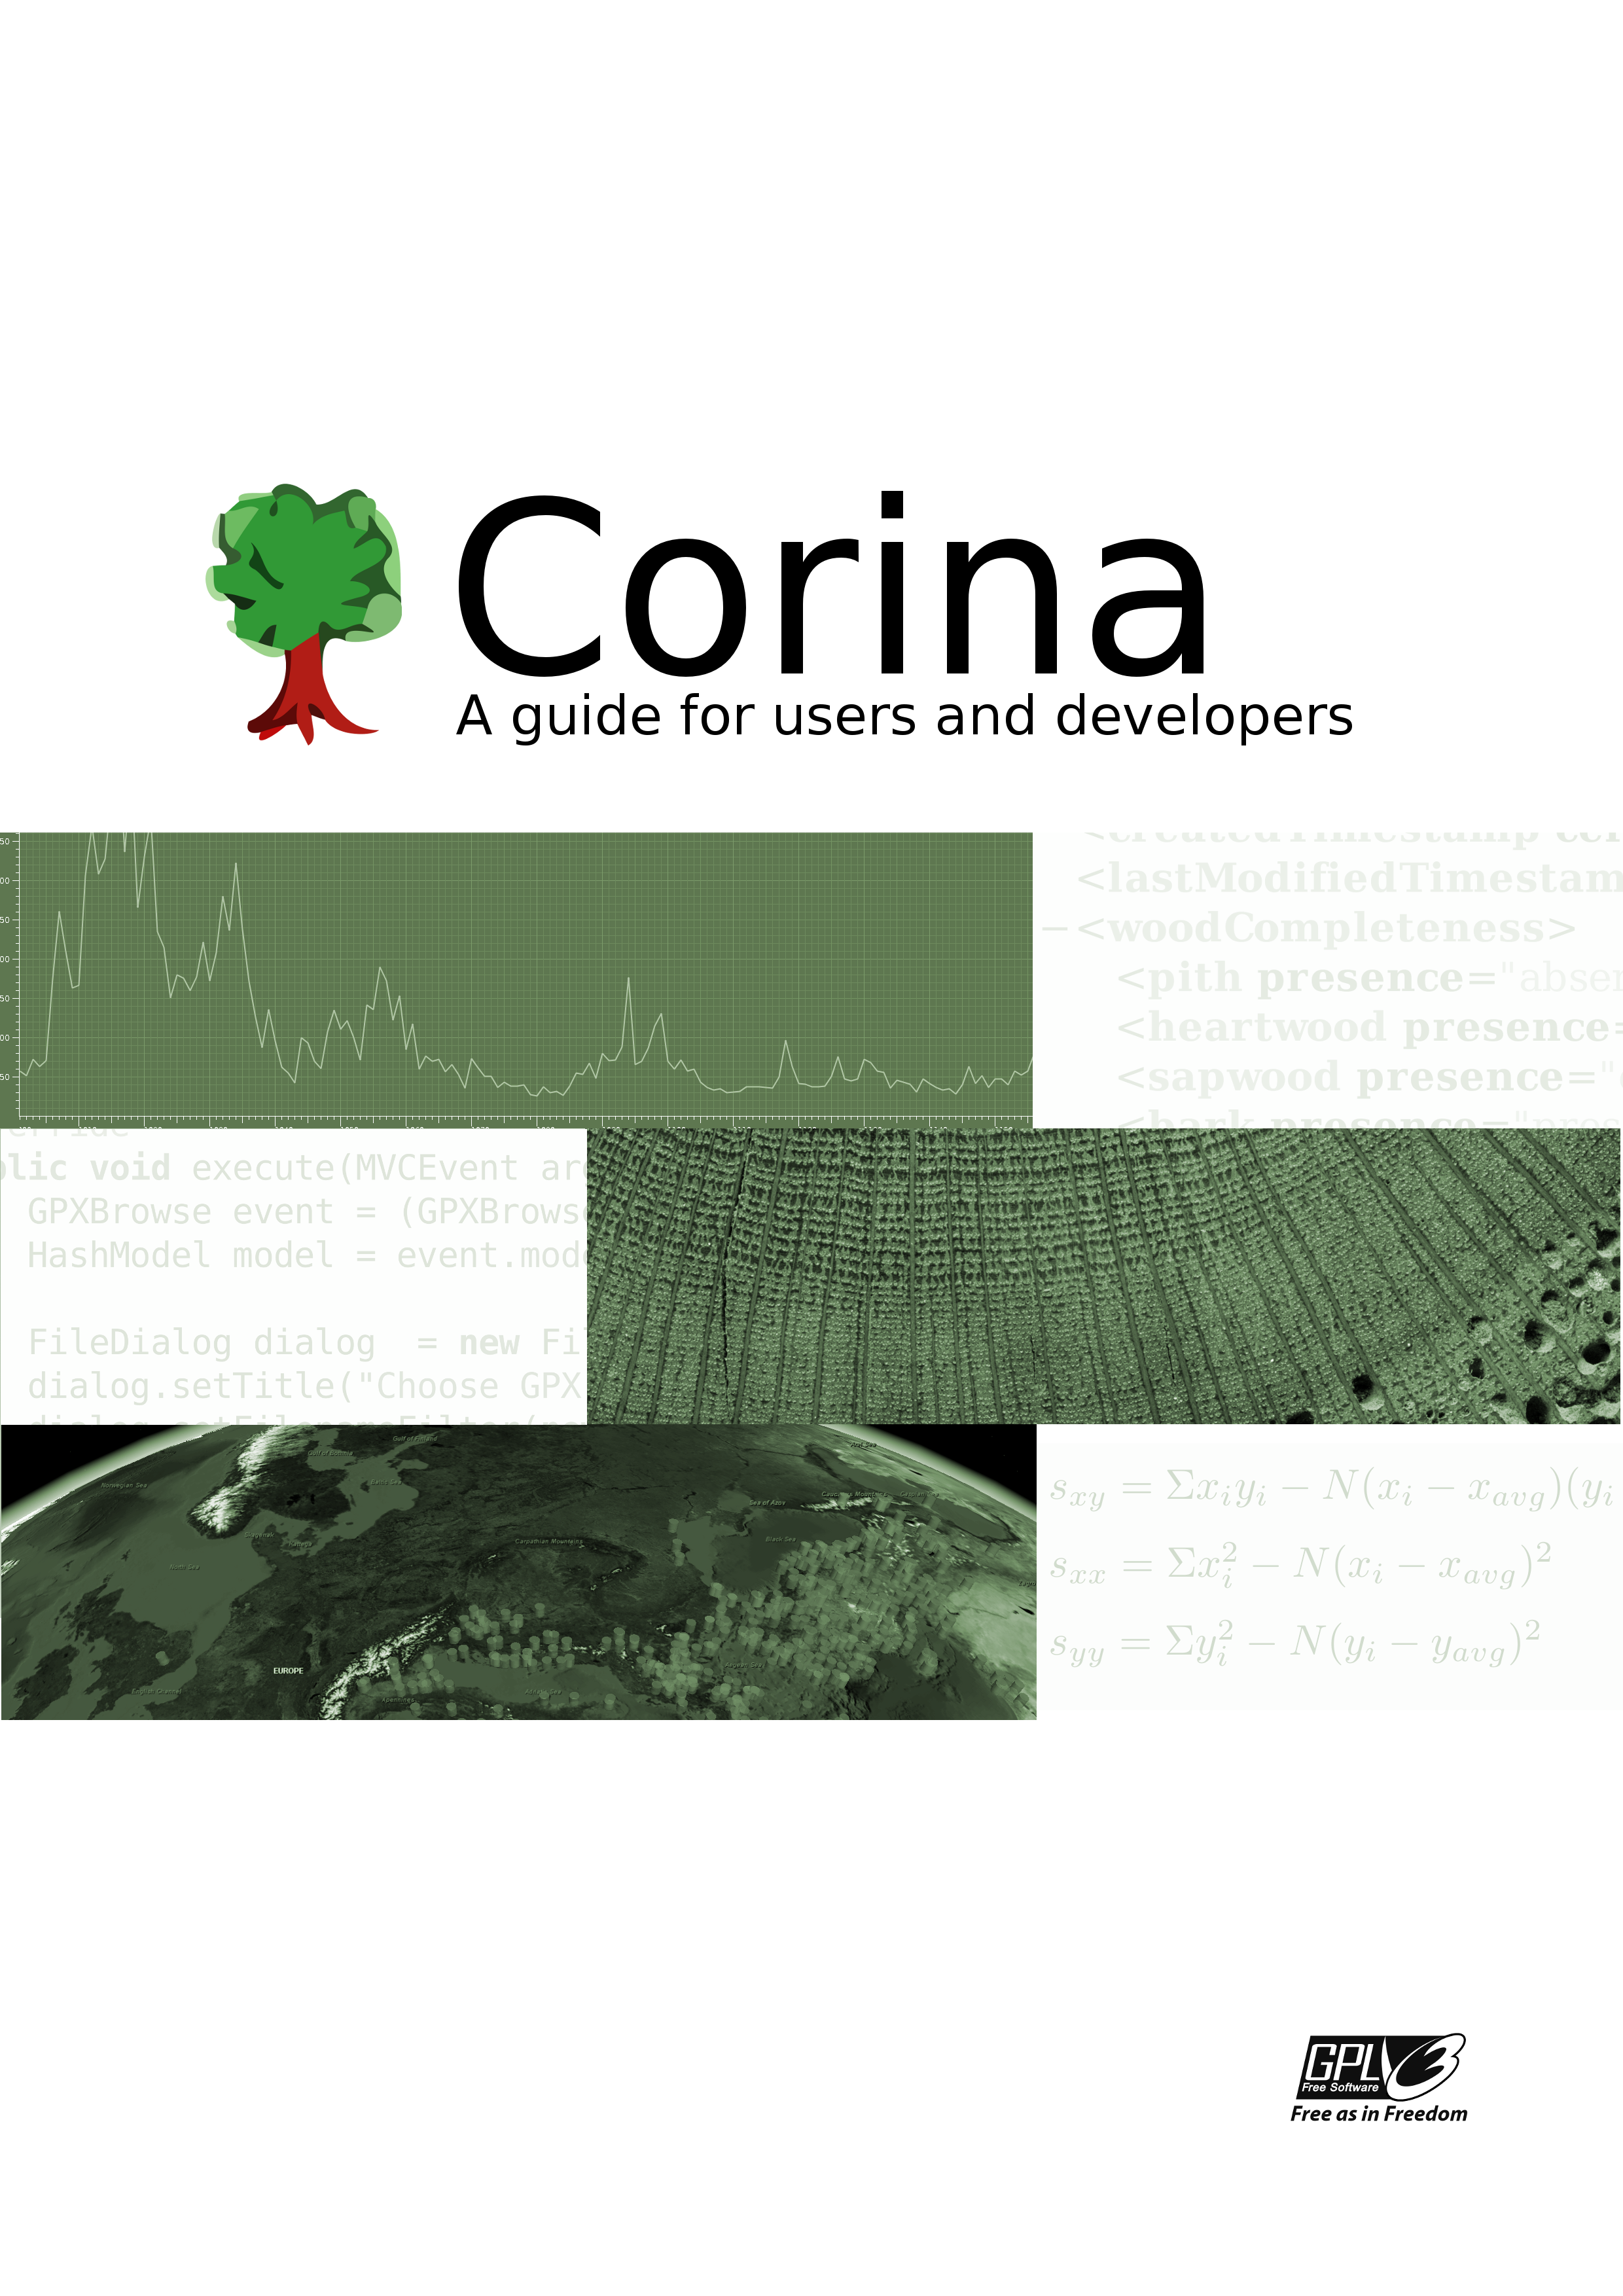
\includegraphics[width=\paperwidth,
keepaspectratio]{Images/background2.png}%
\vfill
}}}



%% Set up headers
\usepackage{fancyhdr}
\setlength{\headheight}{15pt}
\pagestyle{fancyplain}
\renewcommand{\chaptermark}[1]{\markboth{{#1}}{}}
\renewcommand{\sectionmark}[1]{\markright{{Corina: a guide for users and developers}}{}}
\fancyhf{}
\lhead[\fancyplain{}{\thepage}]{}
\chead[\fancyplain{}{\rightmark}]{\fancyplain{}{\leftmark}}
\rhead[]{\fancyplain{}{\thepage}}
\lfoot{}
\cfoot{}
\rfoot{}

%% No headers on empty pages before new chapter
\makeatletter
\def\cleardoublepage{\clearpage\if@twoside \ifodd\c@page\else
    \hbox{}
    \thispagestyle{plain}
    \newpage
    \if@twocolumn\hbox{}\newpage\fi\fi\fi}
\makeatother \clearpage{\pagestyle{plain}\cleardoublepage}



%% Set up code listings
\lstset{ %
basicstyle=\footnotesize,
numbers=left, 
numberstyle=\tiny,
breaklines=true, 
frame=single,
showspaces=false,               % show spaces adding particular underscores
showstringspaces=false,         % underline spaces within strings
showtabs=false,                 % show tabs within strings adding particular underscores
backgroundcolor=\color{lgrey},  % choose the background color. You must add \usepackage{color}
}
